
\chapter{ヒューマニズムの時代}



\section{ガンディー「民主主義と非暴力」(1940)}


マハトマ・ガンディー (Mohandas Karamchand Gandhi, 1869--1848)。

出典:ガンディー『わたしの非暴力』、森達雄訳、みすず書房、1997。

\subsection{}


\emph{問}「どうして貴方は、「民主主義は非暴力によってのみ救われる」とおっしゃるのでしょうか?」(質問者はアメリカの一友人である。)



\emph{答}「なぜなら、民主主義が暴力によって維持されているかぎり、それは弱者を芙蓉し保護することができないからです。民主主義のもとでは、弱者にも最も強い者と同じ機会が与えられるべきであるというのが、わたしの民主主義の考え方です。それは、非暴力による以外はありえません。今日、世界のどんな国も、弱者に対しては横柄な憐みを示すだけです。弱者は負ける、とはよく言われます。ご自身の場合を考えてみてください。あなたがたの所有物は、暴力による以外には維持することはできません{\——}たとえそれが公然とではなく、隠された暴力ではあっても。西洋の民主主義は、いまのところでは、ナチズムやファシズムによって弱められています。そして、せいぜいそれば、ナチやファシストの帝国主義的傾向を隠す仮面になっているにすぎません。もし略奪品を分けるという欲望を満足させるためでなければ、今日どうして戦争があるのでしょうか?英国がインドを手に入れたのは、民主的な方法によったのではありませんでした。南アフリカの民主主義というのは、何のことでしょうか? 南アフリカの憲法そのものが、原住民である有色人種に対して、白人を保護するために作成されたものでした。あなたがたアメリカの歴史は、たぶんそれ以上に不名誉なものです{\——}もっとも、北部諸州が奴隷制の廃止のために努力したことは認められますが。あなたがたの黒人の扱い方は、恥ずべき記録の物語です。しかも、\kenten{そのような民主主義}を救うために、戦争がなされているのです。今日の戦争には、何かひじょうに偽善的な臭いがします。わたしは只今、非暴力の観点から考えています。そして暴力をありのままに曝け出そうと努めているのです。

インドは真の民主化を、すなわち暴力のない民主主義を発展させようと努めています。わたしたちの武器は、\ruby{紡ぎ車}{チャルカ}によって表わされるサティーヤグラハ、農村産業、手仕事を通して教えられる初等教育、不可触賤民制の排除、コミュナル社会の融和、禁酒、アフマダーバードにおけるような非暴力の労働組合などです。それには大衆の努力と、大衆教育が大きな意味をもちます。わたしたちは、こうした活動を行なう大きな機関をもっています。しかもその機関は、全く自発的であり、それのただ一つの認可は、最も身分の賤しい者に奉仕することです。

これは非暴力の努力の永遠の役割です。この努力から、一般に非協力運動とか一般民衆的不服従と呼ばれている、非暴力の抵抗を企てる\ruby{能力}{のうりょく}が生み出されるのです。そしてその運動は、ついには地代や税金の支払いを民衆がこぞって拒否するまでに発展します。ご存知の通り、わたしたちは、かなり大規模に、またかなりうまく非協力と民衆的不服従を試みてきました。その実験には、かがやかしい未来が約束されています。いままでのところ、わたしたちの抵抗はまだ弱者の抵抗ではありましたが、その目標は、強者の抵抗を展開することです。あなたがたの戦争は、けっして民主主義の安全を保証しないでしょう。これに対して、インドの実験は、もし人民が期待に添えるようになってくれれば、別の言葉で言いかえると、もし神がわたしに実験を実らせるのに必要な知恵と力とを与えてくださるなら、民主主義の安全を保証することできますし、またそうすることでしょう。
\begin{flushright}
  1940年5月13日 セヴァグラーム \\
『ハリジャン』1940年5月18日号
\end{flushright}


  \begin{figure}[htbp]
    \centering
      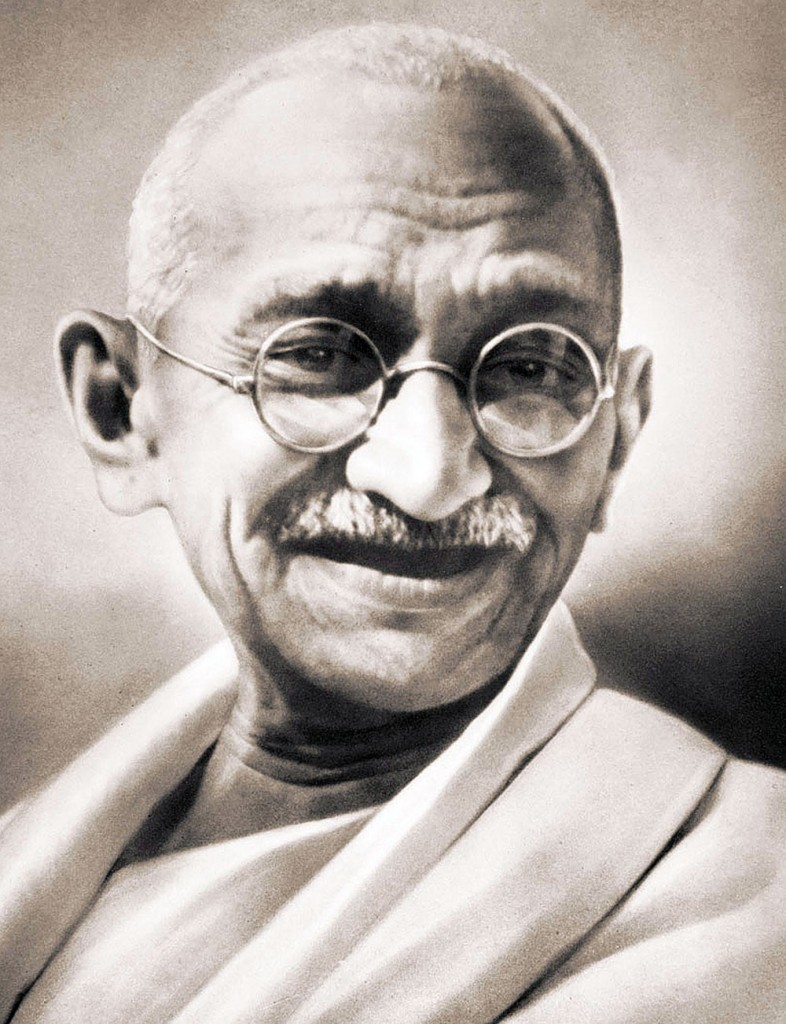
\includegraphics[width=50mm]{images/gandhi.jpg}
    \caption{ガンディー}
  \end{figure}



\newpage{}

\section{サルトル『実存主義とは何か』(1946)}


典拠:J-P・サルトル(1996)『実存主義とは何か』、伊吹武彦訳、人文書院。

\subsection{}


事を複雑にしているのは、実存主義者に二種類あるということである。第一のものはキリスト教信者であって、そのなかにカトリックを信じるヤスパースやガブリエル・マルセルをいれることができよう。第二は無神論的実存主義者で、そのなかにはハイデッガーやまたフランスの実存主義者、そして私自身をいれねばならぬ。この両者に共通なことは、「実存は本質に先立つ」と考えていることである。あるいはこれを、「主体性から出発せねばならぬ」といいかえてもよかろう。このことを正確にはどう理解すべきであろうか。
 たとえば書物とかペーパー・ナイフのような、造られたある一つの物体を考えてみよう。この場合、この物体は、一つの概念を頭にえがいた職人によって造られたものである。職人はペーパー・ナイフの概念にたより、またこの概念の一部をなす既存の製造技術{\——}けっきょくは一定の製造法{\——}にたよったわけである。したがってペーパー・ナイフは、ある仕方で造られる物体であると同時に、一方では一定の用途をもっている。この物体が何に役立つかも知らずにペーパー・ナイフを造る人を考えることはできないのである。ゆえに、ペーパー・ナイフにかんしては、本質{\——}すなわちペーパー・ナイフを製造し、ペーパー・ナイフを定義しうるための製法や性質の全体{\——}は、実存に先立つといえる(39-40)


\subsection{}

実存が本質に先立つとは、この場合何を意味するのか。それは、人間はまず先に実存し、世界内で出会われ、世界内に不意に姿をあらわし、そのあとで定義されるものだということを意味するのである。実存主義の考える人間が定義不可能であるのは、人間が最初は何ものでもないからである。人間はあとになってはじめて人間になるのであり、人間はみずからつくったところのものになるのである。このように、人間の本性は存在しない。その本性を考える神が存在しないからである。人間は、みずからそう考えるところのものであるのみならず、みずから望むところのものであり、実存してのちにみずから考えるところのもの、実存への飛躍ののちにみずから望むところのもの、であるにすぎない。人間はみずからつくるところのもの以外の何ものでもない。以上が実存主義の第一原理なのである。これがまたいわゆる主体性であり、まさしくそのような名で世人がわれわれに非難しているものなのである。しかしわれわれがそれによって意味するのは、人間は石ころや机よりも尊厳であるということ以外にはない。というのは、われわれは人間がまず先に実存するものだということ、すなわち人間はまず、未来にむかって自らを投げるものであり、未来のなかにみずからを投企することを意識するものであることをいおうとするのだからである。(42)

\subsection{}

われわれが、人間はみずからを選択するというとき、われわれが意味するのは各人がそれぞれ自分自身を選択するということであるが、しかしまた、各人はみずからを選ぶことによって、全人類を選択するということをも意味している。じっさい、われわれのなす行為のうち、われわれがあろうと望む人間をつくることによって、同時に、人間はまさにかくあるべきだとわれわれの考えるような、そのような人間像をつくらない行為は一つとしてない。あれかこれか、そのいずれかであることを選ぶのは、われわれが選ぶそのものの価値を同時に肯定することである。というのは、われわれはけっして悪を選びえないからである。われわれが選ぶものはつねに善であり、何ものも、われわれにとって善でありながら万人にとって善でない、ということはありえないのである。他方、もし実存が本質に先立つものとすれば、そしてわれわれが、われわれ自身の像をつくり実存しようと欲するなら、この像は万人のために、そしてわれわれの時代全般のために有効である。このように、われわれの責任は、われわれが想像しうるよりもはるかに大きい。われわれの責任は全人類をアンガジェするからである。もし私が労働者であり、コミュニストであるよりもむしろキリスト教的シンジケートに加盟することを選び、この加盟によって、諦めがけっきょくは人間にふさわしい解決であり、人間の王国は地上には存在しないことを示そうとすれば、私はたんに私一個人をアンガジェするのではない。私は万人のために諦めようとするのであり、したがって私の行為は人類全体をアンガジェしたことになる。もっと個人的なことであるが、もし私が結婚し、子供をつくることを望んだとしたら、たとえこの結婚がもっぱら私の境遇なり情熱なり欲望なりにもとづくものであったとしても、私はそれによって、私自身だけでなく、人類全体を一夫一婦制の方向へアンガジェするのである。こうして私は、私自身にたいし、そして万人にたいして責任を負い、私の選ぶある人間像をつくりあげる。私を選ぶことによって私は人間を選ぶのである。(44-45)

\subsection{}


ドストエフスキーは、「もし神が存在しないとしたら、すべてが許されるだろう」と書いたが、それこそ実存主義の出発点である。いかにも、もし神が存在しないならすべてが許される。したがって人間は孤独である。なぜなら、人間はすがりつくべき可能性を自分のなかにも自分のそとにも見出しえないからである。人間はまず逃げ口上をみつけることができない。もしはたして実存が本質に先立つものとすれば、ある与えられ固定された人間性をたよりに説明することはけっしてできないだろう。いいかえれば、決定論は存在しない。人間は自由である。人間は自由そのものである。もし一方において神が存在しないとすれば、われわれは自分の行いを正当化する価値や命令を眼前に見出すことはできない。こうしてわれわれは、われわれの背後にもまた前方にも、明白な価値の領域に、正当化のための理由も逃げ口上ももってはいないのである。われわれは逃げ口上もなく孤独である。そのことを私は、人間は自由の刑に処せられていると表現したい。刑に処せられているというのは、人間は自分自身をつくったのではないからであり、しかも一面において自由であるのは、ひとたび世界のなかに投げだされたからには、人間は自分のなすこと一切について責任があるからである。(50-51)

\subsection{}


おわかりにように、この主義は人間を行動によって定義するものである以上、これを静寂主義の哲学と考えるわけにはいかない。また人間の悲観論的記述とも考えられない。人間の運命は人間自身のなかにある以上、これほど楽観的な主義はないからである。また人間にむかって、希望は彼の行動のなかにしかなく、人間を生かす唯一のものは行為であると説くのであるから、行動にたいして人間を絶望させるための試みと考えることもできない。したがってこの面においては、これは行動とアンガジュマンのモラルである。しかも人々は、これらいくつかの与件から出発して、われわれが人間を個々の主体性にとじこめるものだと非難する。その点でも人々はわれわれを非常に誤解している。なるほどわれわれの出発点は個人の主体性であるが、これは厳密に哲学的な理由によるのである。われわれがブルジョアだからではなく、真理にもとづく主義を欲するからであり、希望に満ちてはいるが現実的基礎をもたぬ結構な学説の集積を望んではいないからである。出発点において、「われ考う、故にわれあり」という真理以外の真理はありえない。これこそ、自分自身を捉える意識の絶対的真理である。人間が自分自身を捉えるこの瞬間のそとに人間を把握するすべての学説は、何よりもまず、真理を抹殺する学説である。というのは、このデカルト的コギトを外にして、あらゆる対象はただ蓋然的であるにすぎず、真理によりかからぬ蓋然性の学説は無のなかに崩壊してしまう。蓋然的なものを定義するには、真なるものをもっていなければならない。したがってある真理が存在するためには絶対的真理が必要である。そして絶対的真理は簡単であり捉えやすい。それは仲介なしに自己を捉えることにある。

第二にこの学説は、尊厳さをあたえる唯一のもの、人間を物体視しない唯一の学説なのである。すべて唯物主義はその結果として、自己をふくめるあらゆる人間を物質として扱う。すなわち、机や椅子や石を構成する性質や現象の全体となんの区別もない一定の反応の全体として取り扱う。われわれはまさに人間界を、物質界とは区別された諸価値の全体として構成しようと望むのである。しかしわれわれがここに真理として到達する主体性は、厳密に個人的な主体性ではない。というのは、われわれは、コギトのなかに自分自身だけをでなく他者をも発見することを証明したからである。デカルトの哲学とは反対に、またカントの哲学とは反対に、われわれは「われ考う」によって、他者の面前でわれわれ自身を捉える。そして他者はわれわれにとって、われわれ自身と同様に確実なのである。こうして、コギトによって直接におのれを捉える人間は、すべての他者をも発見する。しかも他者を自己の存在条件として発見するのである。彼は他者がそうと認めないかぎり(彼は機知に富むとか、意地が悪いとか、嫉妬ぶかいとか人がいうその意味で)自分が何ものでもありえないことを理解している。私にかんしてのある真実を握るためには、私は他者をとおってこなければならない。他者は、私が自分にかんしてもつ認識に不可欠であるとともに、私の存在にとっても不可欠である。こうした状態において、私の内奥の発見は同時に他者を、私の面前に置かれた一つの自由、私に同調しまた反対してしか考えずまた意志しない一つの自由として私に発見させる。こうしてわれわれは、ただちに、相互主体性とわれわれの呼ぶ一つの世界を発見する。人間はこの世界においてこそ、現に自分があるところのものと、他者があるところのものとを決定するのである。(64-66)


\begin{figure}[htbp]
  \centering
     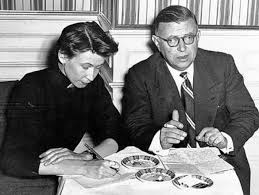
\includegraphics[width=70mm]{images/sartre-beauvoir.jpg}
  \caption{サルトルとボーヴォワール}
\end{figure}

\newpage{}

\section{ボーヴォワールの『第二の性』(1949)}



シモーヌ・ド・ボーヴォワール、井上たか子・木村信子監訳(1997)『決定版 第二の性I:事実と神話』新潮社

\subsection{序文}

ところで、女は男の奴隷ではないまでも、少なくともつねに男の家来であった。男と女が世界を平等に分かちあったことは一度もない。女の地位は向上しつつあるとはいえ、いまなお、女は重いハンディキャップを背負っている。ほとんどの国で、男女の法的身分は同一ではなく、女にとっては非常に不利になっていることが多い。理論的には女にさまざまな権利が認められている場合でも、古くからの習慣が妨げになって、それらの権利が風習のなかで具体的に生かされない。経済面では、男と女はほとんど別のカースト〔階級とは異なり、固定的で閉鎖された社会集団〕を構成している。条件はまったく同じでも、男たちは、新参の競争相手である女よりも有利な地位につき、給料も高く、出世のチャンスも多い。男たちは、産業界、政界その他で、女よりはるかに多くの場所を占め、しかもいちばん重要なポストは彼らが握っている。男には、こうした具体的な権力に加えて、子どものときの教育全体を通じて伝統として守られている威信が身についている。現在には過去が含まれており、過去において歴史はすべて男によってつくられてきたからだ。今では女も世界の建設に参加しはじめているが、この世界はまだ男の世界である。男はそれに疑問をもたず、女もほとんど疑問を感じない。仮に女が〈他者〉であることを拒否したり、男との共犯関係を拒否したりすれば、それは女にとって、上層カーストとの同盟が与えてくれる特典をすべてあきらめることになるだろう。主君である男の家来でいれば、男は女を物質的に保護し、その存在の意味づけまで引き受けてくれるはずだ。こうして女は、経済的な危険だけでなく、自らの目的を独力で見つけなくてはならない自由な存在につきものの形而上学的な危険をも回避する。実際、どんな人間にもそれぞれ自分を主体として主張したいという倫理的な欲求とならんで、自由を逃れてモノになりたいという気持ちがあるからだ。だが、これは不幸な道である。なぜなら、受動的で、疎外され、自分を見失った人間は、超越への道を断たれ、あらゆる価値をだまし取られて、他人の意志の餌食になってしまうからだ。けれども、これは楽な道でもある。この道をとれば、各自が本来的に引き受けるべき実存の不安と緊張を避けることができる。したがって、女を〈他者〉と定める男は、女の奥底にひそむ共犯性に気づくはずである。このように、女は自分を主体として主張しない。それは、そのための具体的な手段をもっていないからであり、自分を男に結びつけている絆を不可欠のものと感じ、その絆の相互性を認めていないからであり、たいていは〈他者〉という自分の役割に満足しているからである。(I, 15-17)



\subsection{歴史}


女のことで生じる根本的な問題の一つは、すでに見たように、生殖の役割と生産労働をどう両立させるかということである。歴史の始まりには女は家事をするものと決められ、世界の建設への参加を禁じられた根深い理由は、女が生殖機能に縛りつけられていることだった。動物の雌には発情期と活動期のリズムがあって体力が蓄えられるようになっている。ところが、思春期から更年期までのあいだずっと自然は女の妊娠能力を制限していない。早婚を禁止している文明もあり、次の出産までに少なくとも二年の休息を女に保証することを義務づけているインディアン部族の例もあるが、全般的には何世紀ものあいだ女の受胎能力は調整されなかった。古代から、水薬、座薬、膣用タンポンなど、主に女が使用するための避妊方法はあったが、それらはずっと売春婦と医者の秘密だった。風刺作家たちは頽廃期のローマの女たちの不妊をとがめているが、彼女たちはおそらくこの秘密を知っていたのだろう。しかし、中世になると避妊方法は知られず、十八世紀にいたるまでその痕跡は何も見つかっていない。こうした時代には、多くの女の人生は絶えまない妊娠の連続だった。身持ちのよくない女も、何度も母親になることで、愛のたわむれにつけを払わなければならなかった。時代によっては人類は人口を減らす必要を痛感したが、同時に国家はそれによって弱体化するのを恐れた。危機や貧困の時代に出生率の低下が実現したのは、独身者の結婚年齢が上がったためである。〔……〕フランスでマルサス主義的傾向が拡大するのは十八世紀になってからである。まず裕福な階級が、続いて国民全体が、両親の財力に応じて子どもの数を制限するのは理にかなったことだと考え、避妊方法が生活習慣にとりいれられ始める。〔……〕フランスでは避妊の宣伝やベッサリー、膣用タンポンなどの販売は禁止されているが、それでも「バースコントロール」は普及している。

妊娠中絶の方は法律によって公認されたところはどこにもなかった。ローマ法は、胎児の生命に対する特別な保護は認めていなかった。胎児を人間としてではなく、母体の一部と見なしていたのだ。「誕生前の子どもは女の一部であり、内臓のようなものである」。ローマ帝国の頽廃期には中絶は正規の医療行為と見なされ、立法者は出産を奨励したかったときも、あえて中絶を禁止しなかった。妻が夫の意に反して子どもを拒否したときは、夫は妻を処罰させることができた。しかしその場合、犯罪に相当したのは妻の不服従だった。オリエント文明およびギリシア・ローマ文明全体を通じて、中絶は法律で認められていた。(I, 173-175)

〔……〕慣習が独身女性に独身男性と同等の性的可能性を認めるには、まだほど遠い。とくに独身女性が子どもを産むことはほとんど禁じられていて、未婚の母はいまだスキャンダルの対象である。シンデレラの神話はなくならないだろう。誰もが今でも若い娘に、「すてきな王子さま」に幸運と幸福を期待する方が、一人でそれを手に入れようと困難で不確かな試みをするよりもいいとすすめている。とくに、娘は王子によって自分のカーストよりも上のカーストに上昇することを期待できる。それは彼女が一生働いても与えられない奇跡である。しかし、そういう望みは彼女の努力と利益を分裂させてしまうので有害である。女にとって最も大きいハンディキャップは、おそらくこの分裂である。両親はいまでも娘を、その個性をのばすよりも、結婚させるために育てている。娘もその方が有利だと思って、自分からそれを望むほどだ。その結果、娘の大部分はその兄弟ほど専門技術を身につけず、しっかりした教育も受けず、自分の職業に全身全霊で打ち込むこともしない。そのためにいつまでも低い地位にあまんじることになる。そして悪循環が始まる。この劣等意識が夫を見つけたいという願望を強めるのだ。利益の裏側にはいつも負担がともなっている。そして、その負担が重すぎると利益も拘束としか思えない。大多数の労働者にとっていま労働はやりがいのない苦役であり、しかも女にとってはその苦役が、社会的栄誉や、慣習からの解放、経済的自立などの具体的獲得によって償われることがない。女子工員や女子事務員の多くが働く権利のなかに義務しか見出せないので、結婚すればそこから解放されると思うのも当然なのだ。とはいえ、女はすでに自意識をもち、仕事によって結婚から解放されることもできるので、これまでのようにおとなしく結婚への服従を受け入れたりもしない。女が望むのは、家庭生活と職業を両立させるのに身をすり減らすような離れ業を必要としないことである。それにしても、安易さへの誘惑があるかぎり{\——}経済的不平等が一部の人間を有利にし、そうした特権者の誰かに身を売る権利が女に認められているだけに{\——}女が自立への道を選ぶためには、男より大きな精神的努力を必要とするだろう。(I, 196-197)

\subsection{神話}


しかし、もっと一般的に男の心にあるのは、自分の肉体的条件に対する反抗である。男は自分を失墜した神だと思っている。男の宿命的な不幸は、輝かしい天空から墜落して、母親の腹という混沌とした闇に入れられたことだ。男が自分の姿を認めたがっているあの火、活発で純粋なあの息吹、女はこれを大地の泥に閉じ込める。男は〈一者〉〈全体〉〈絶対精神〉のように、純粋〈理念〉として必然でありたいと思う。それなのに、限られた身体のなかに、自分が選んだわけでなく呼ばれたわけでもない時間と場所のなかに閉じ込められて、役立たずで、場所塞ぎで、不条理だ。肉体の偶然性は男の存在そのものの偶然性であり、男は見捨てられて、許しがたい無根拠性のなかで、この偶然性にさらされる。偶然性は男を死にも捧げる。〔……〕男は無根拠性と死が嫌いだから、自分が生み出されたことが気に入らない。(I, 208-209)

神話にはさまざまな種類がある。女の神話は、人間が男女二つのカテゴリーに「区分」されているという、人間の条件の一つの不変的な側面を純化したものであり、静的な神話である。女の神話は、経験のなかで捉えられた現実、あるいは経験に基づいて概念化された現実を、プラトン的な天空に投影している。事実や価値、意味、概念、経験的法則を、超越的、非時間的、不変的、必然的な〈イデア〉に置き換えているのだ。こうした概念は、経験的な事実を超えたところに位置づけられていて、いかなる異論の余地もない。もともと絶対的な真理をそなえているのだ。このように、神話的な思考は、あらゆる女たちの分散的、偶然的、多面的な実存に、唯一の固定した〈永遠の女性的なるもの〉を対置させる。〈永遠の女性的なるもの〉に与えられる定義が生身の女たちの行為と食いちがっているときは、いつでも女たちの方が間違っていることになる。〈女らしさ〉とは観念の産物にすぎないと宣告するかわりに、女たちの方が女らしくないと宣言されるのだ。(I, 337)


\subsection{子ども時代}



人は女に生まれるのではない、女になるのだ。社会において人間の雌がとっているのは生理的宿命、心理的宿命、経済的宿命のどれでもない。文明全体が、男と去勢者の中間物、つまり女と呼ばれるものを作りあげるのである。他人の介在があってはじめて個人は〈他者〉となる。子どもは自分に対してだけ存在しているかぎりは、自分を性的に異なるものとしてとらえることはできない。女の子、男の子にあっては、身体はまず主体性の輝かしい発現、世界を理解するための道具である。彼らが世界をとらえるのは目や手をとおしてであって、性器をとおしてではない。出生、離乳のドラマは乳児にとって男女とも同じように展開する。男女の乳児ともに同じ興味、同じ喜びを感じるのだ。〔……〕少女が思春期のかなり前から、またときには幼い頃から、性的に特定化されているように見えるのは、不思議な本能によって少女が受動性、媚び、母性へと直接運命づけられているからではない。子どもの生活には、ほぼ最初から他人が介在していて、生まれたばかりの頃から子どもにその使命が強制的に吹き込まれるからである。(II, 11-12)

\subsection{結婚した女}


このように、女が家庭内で行なっている労働は女に主体性を与えはしない。この労働は直接的に共同体の役に立つこともなく、未来に通じてもいないし、何も生み出しはしない。この労働が意味と尊厳をもつのは、生産あるいは行動において社会へ向けて自己を超越する存在に同化された場合だけである。つまり、この労働は既婚女性を解放するどころか、夫や子どもに従属させるのである。夫や子どもを通じて彼女は自己証明する。彼女は非本質的な媒介物として彼らの人生にかかわっているにすぎないのだ。民法典は妻の義務から「服従」を削除したが、それでも妻の状況はまったく変化していない。妻の状況は夫の意志にかかっているのではなく、夫婦共通財産制という構造そのものにかかっているのである。女には建設的な仕事をなすことが許されておらず、したがって自分が完成した人格であることを明らかにすることが許されていない。尊敬されるにしても、女は従属者、脇役、寄生者なのだ。女に重くのしかかっている大きな不運は、自分の存在の意味そのものが自分の手に握られていないことである。だからこそ、結婚生活の成功、失敗が男より女にとってずっと重みをもつのだ。男は夫である前に市民、生産者である。女は何よりもまず、そしてたいていはもっぱら、妻である。女の労働は女を女の条件から救い出しはしない。逆に、女の労働が女の条件から女の労働の価値を引き出したり引き出さなかったりするのだ。愛情に満ちていて、惜しみなく献身していれば、女は嬉々として任務を果たすだろう。恨みをいだきながら任務を行なっていれば、それは女に無味乾燥な苦役に思えるだろう。女の任務は要するに女の人生において非本質的な役割しかもたない。結婚生活の災難のなかで、女の任務は頼りにはならない。(II, 261-262)

\subsection{自立した女}


現在、自由に行使することがほとんど不可能な女の機能が一つある。それは母性だ。イギリスやアメリカでは、女は少なくとも「バースコントロール」実施のおかげで、自分の意志で出産を拒否できる。すでに見てきたように、フランスでは、女は苦しくかつ費用のかかる中絶に追いこまれる場合がしばしばある。たいていは、望んで産んだのではない子どもの面倒を女が引き受け、自身の職業生活を失うことになる。その負担が重いのは、慣習が逆に、女が望むときに妊娠できるようにさせていないからだ。未婚の母はスキャンダルとなり、子どもにとっても婚外子ということは大きな欠陥となる。結婚の束縛を受け入れずに、または身をもちくずさずに、母親になれるのは稀である。人工授精の考えが多くの女の関心を引くのは、彼女たちが男の抱擁を避けたいと思っているからではない。社会によって自由な母性がついには認められるようになることを願っているからだ。補足しなくてはならないが、きちんと組織された託児所や幼稚園がなかったら、子どもが一人いるだけで、女の活動は完全に身動きがとれなくなる。子どもを親や友人や家政婦に任せることでしか自分の仕事を続ける道はない。彼女は、つらい欲求不満を感じさせる不妊か、職業生活との両立がむずかしい負担を引き受けるか、どちらかを選ばなくてはならない。(II, 579-580)

\subsection{結論}


〔……〕とはいえ、女が変わるには、その経済的な条件を変えるだけですむと思ってはならない。経済的要因は、たしかに、女を変えるのに基本的なものだったし、今もそうだろう。しかし、この要因が生みだすと同時に必要ともしている精神的、社会的、文化的な成果がついてこなかったら、新しい女は生まれないだろう。今のところ、そうした成果は、どこにも、ソ連にも、フランスにも、アメリカにも、実現されていない。そのせいで、今日の女は過去と未来のあいだで引き裂かれている。今日の女は、たいていの場合、男に変装した「ほんとうの女」のように見え、自分の女としての身体のなかでも、その男っぽい衣服のなかでも居心地悪そうにしている。女は、生活を一新し、自分にあった服装を身につける必要がある。それは集団が変化しなければできないことだろう。今日、どんな教育者も、一人では、「男の人間」とまったく同等の「女の人間」をつくることはできない。女の子は、男の子のように育てられれば、自分が例外だと思うだろうし、そうなれば、また新しい種類の差別を受けることになる。スタンダールはこうしたことがよくわかっていた。彼は「森林は一気に植えないとだめだ」と言っていた。しかし、もし私たちが、逆に、男女平等の具体的に実現されているような社会を想定できるなら、その平等が個々人のうちに新たに確立されるかもしれないのだ。(II, 614)




 \begin{figure}[htbp]
 \center
      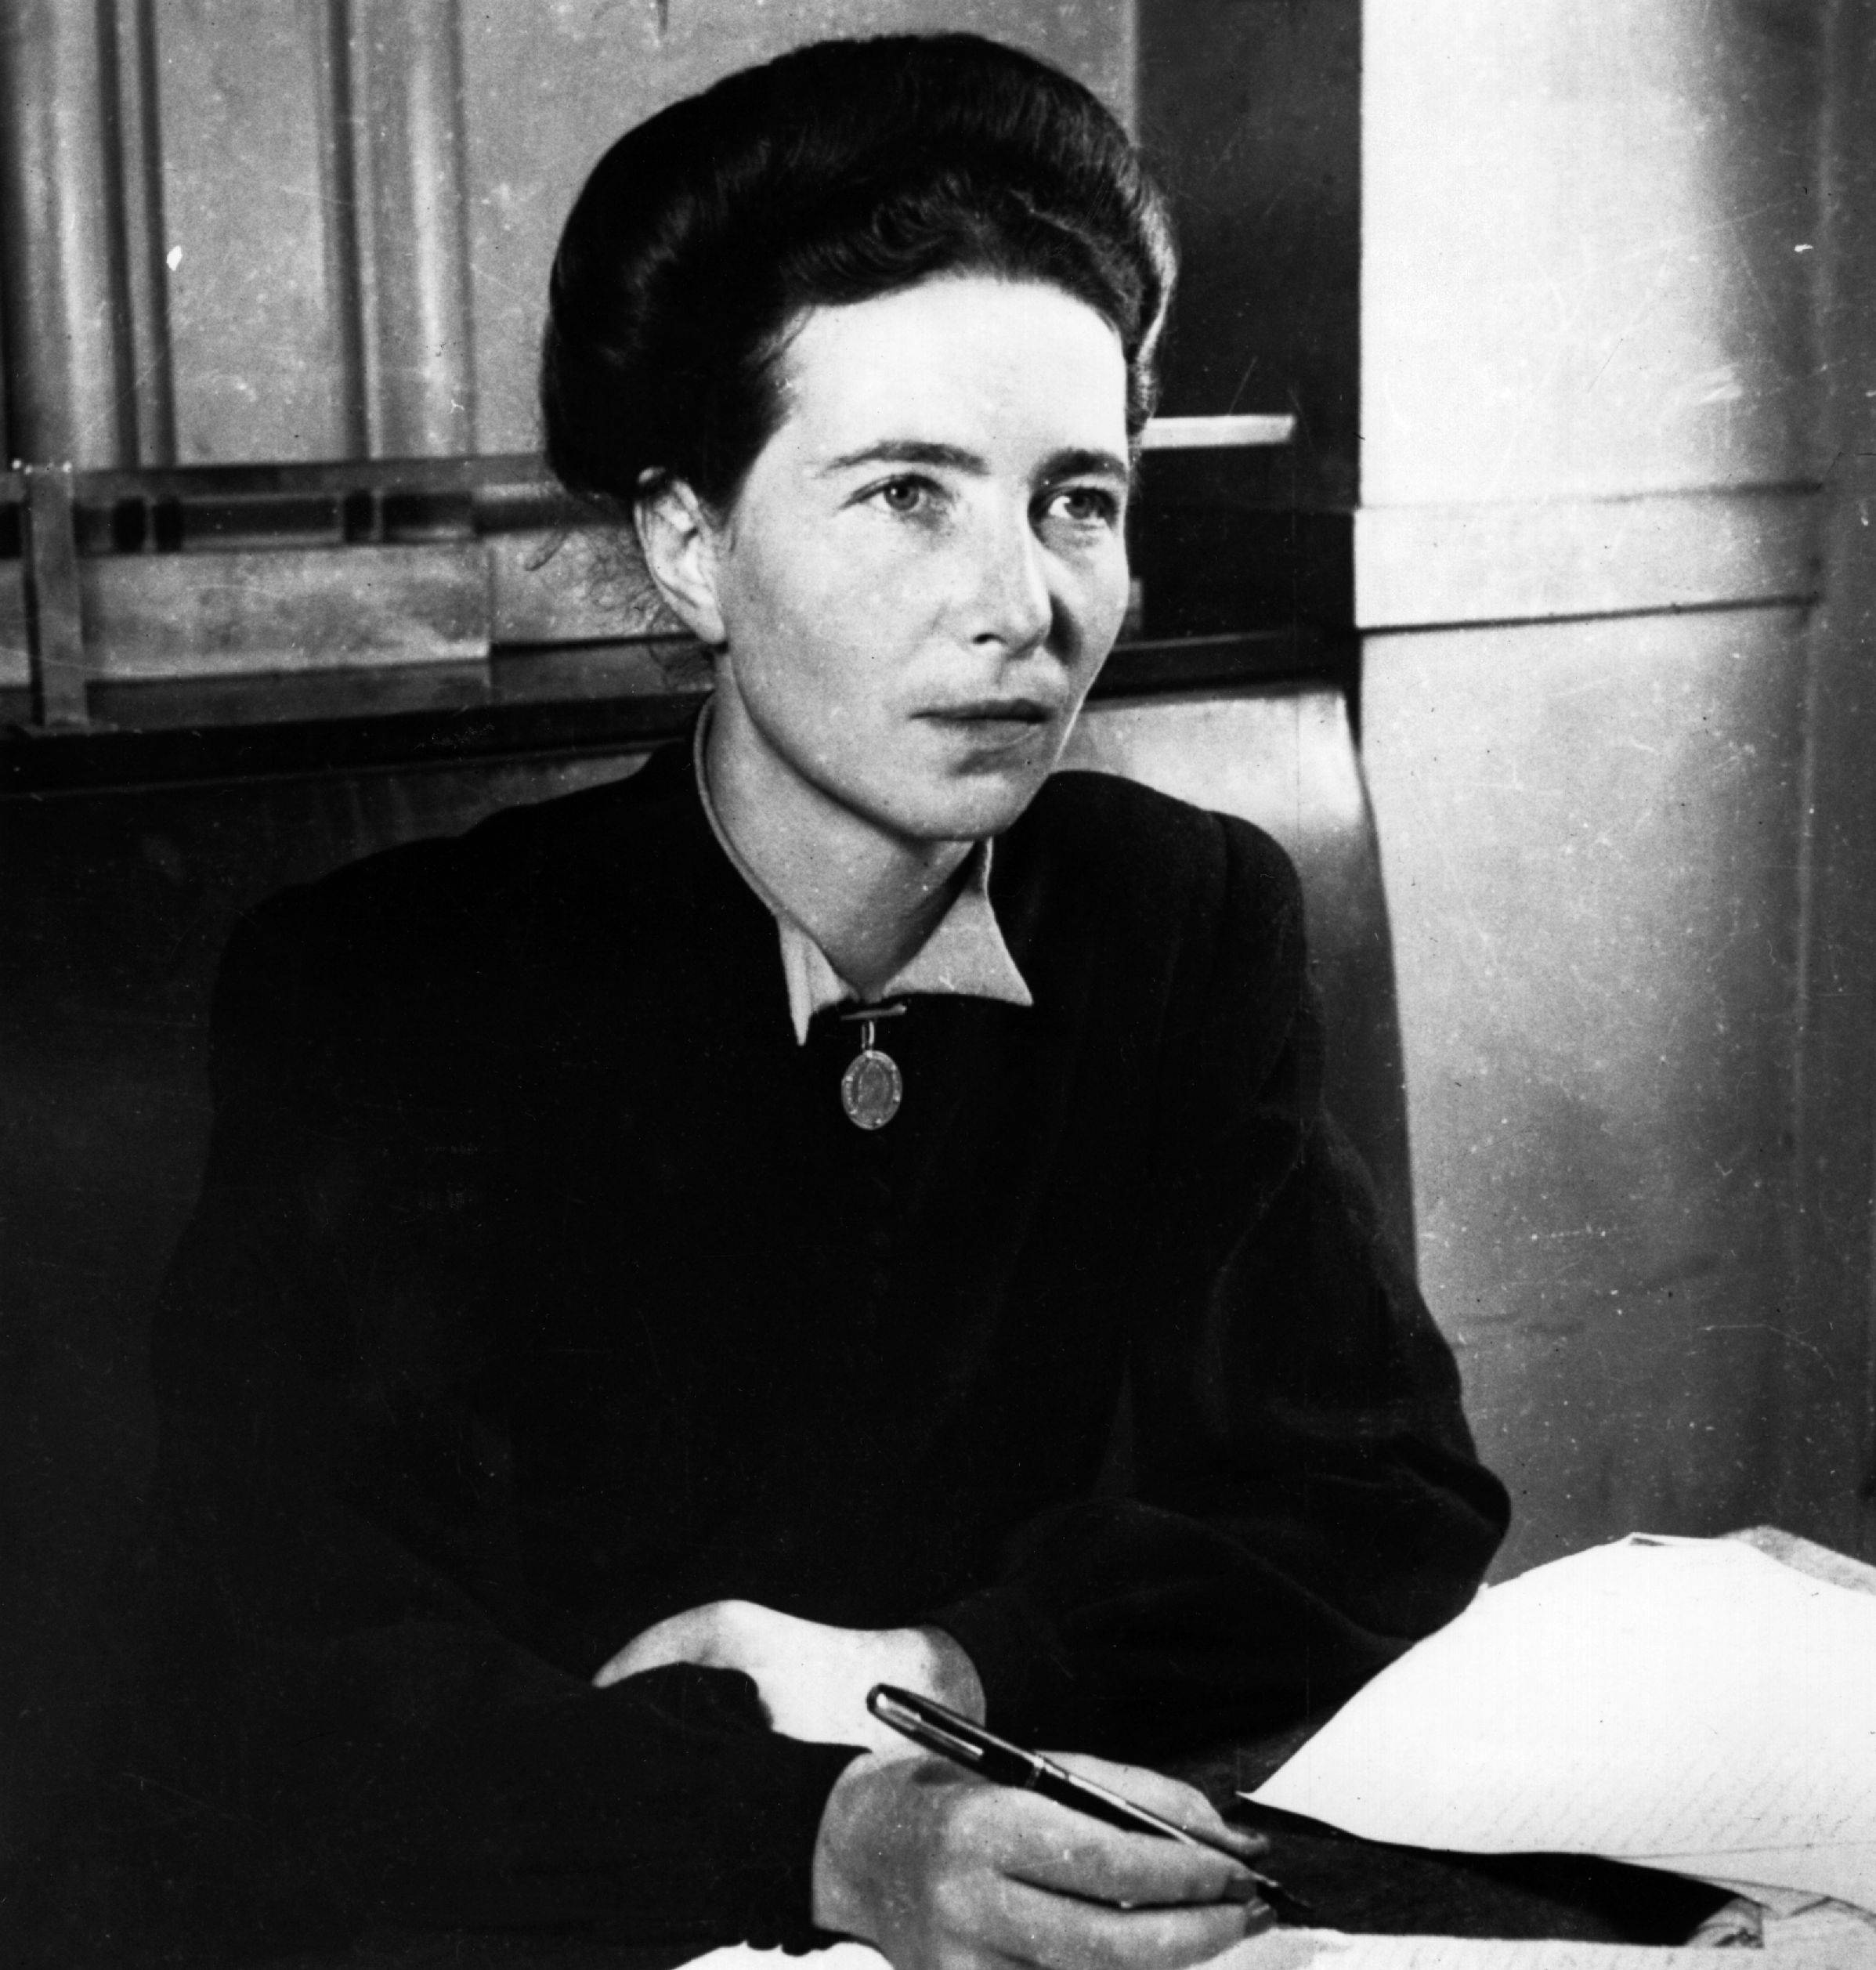
\includegraphics[width=50mm]{images/beauvoir.jpg}
   \caption{ボーヴォワール}
 \end{figure}


\section{推薦図書}

\begin{itemize}
\item  アリス・シュヴァルツァー、福井美津子訳(1994)『ボーヴォワールは語る 『第二の性』その後』平凡社。インタビューの記録。「その後」がとても大事。(渡)
\end{itemize}






%%% Local Variables:
%%% mode: japanese-latex
%%% TeX-master: "main_gendai"
%%% coding: utf-8
%%% End:
